\ifdefined\ENGLISH
\newcommand{\GlobalVarsSectionName}{Global variables}
\section{\GlobalVarsSectionName}
\myindex{\GlobalVarsSectionName}
\label{scanf_global_variable}

What if the \TT{x} variable from the previous example was not local but a global one? 
Then it would have been accessible from any point, not only from the function body. 
Global variables are considered \gls{anti-pattern}, but for the sake of the experiment, we could do this.
\fi

\ifdefined\RUSSIAN
\newcommand{\GlobalVarsSectionName}{Глобальные переменные}
\section{\GlobalVarsSectionName}
\myindex{\GlobalVarsSectionName}
\label{scanf_global_variable}

А что если переменная \TT{x} из предыдущего примера будет глобальной переменной, а не локальной? 
Тогда к ней смогут обращаться из любого другого места, а не только из тела функции. 
Глобальные переменные считаются \glslink{anti-pattern}{анти-паттерном},
но ради примера мы можем себе это позволить.
\fi

\ifdefined\BRAZILIAN
\newcommand{\GlobalVarsSectionName}{Variáveis globais}
\section{\GlobalVarsSectionName}
\myindex{\GlobalVarsSectionName}
\label{scanf_global_variable}

E se a variável \TT{x} do último exemplo não fosse local, mas sim global?
Então ela teria que ser acessível de qualquer ponto, não somente pelo corpo da função.
Variáveis globais são consideradas maus hábitos, mas pelo bem do experimento, nós faremos isso.
\fi

\lstinputlisting{patterns/04_scanf/2_global/ex2.c.\LANG}

\EN{\subsectionold{MSVC: x86}

\lstinputlisting{patterns/04_scanf/2_global/ex2_MSVC.asm}

In this case the \TT{x} variable is defined in the \TT{\_DATA} segment and no memory is allocated in the local stack. It is accessed directly, not through the stack. 
Uninitialized global variables take no space in the executable file
(indeed, why one needs to allocate space for variables initially set to zero?), 
but when someone accesses their address, 
the \ac{OS} will allocate a block of zeroes there\footnote{That is how a \ac{VM} behaves}.

Now let's explicitly assign a value to the variable:

\lstinputlisting{patterns/04_scanf/2_global/default_value_EN.c}

We got:

\begin{lstlisting}
_DATA	SEGMENT
_x	DD	0aH

...
\end{lstlisting}

Here we see a value \TT{0xA} of DWORD type (DD stands for DWORD = 32 bit) for this variable.

If you open the compiled .exe in \IDA, you can see the \IT{x} variable placed at the beginning of 
the \TT{\_DATA} segment, and after it you can see text strings.

If you open the compiled .exe from the previous example in \IDA, where the value of \IT{x} was not set, you would see something like this:

\begin{lstlisting}
.data:0040FA80 _x              dd ?                    ; DATA XREF: _main+10
.data:0040FA80                                         ; _main+22
.data:0040FA84 dword_40FA84    dd ?                    ; DATA XREF: _memset+1E
.data:0040FA84                                         ; unknown_libname_1+28
.data:0040FA88 dword_40FA88    dd ?                    ; DATA XREF: ___sbh_find_block+5
.data:0040FA88                                         ; ___sbh_free_block+2BC
.data:0040FA8C ; LPVOID lpMem
.data:0040FA8C lpMem           dd ?                    ; DATA XREF: ___sbh_find_block+B
.data:0040FA8C                                         ; ___sbh_free_block+2CA
.data:0040FA90 dword_40FA90    dd ?                    ; DATA XREF: _V6_HeapAlloc+13
.data:0040FA90                                         ; __calloc_impl+72
.data:0040FA94 dword_40FA94    dd ?                    ; DATA XREF: ___sbh_free_block+2FE
\end{lstlisting}

\TT{\_x} is marked with \TT{?} with the rest of the variables that do not need to be initialized. 
This implies that after loading the .exe to the memory, a space for all these variables is to be 
allocated and filled with zeroes [\CNineNineStd 6.7.8p10].
But in the .exe file these uninitialized variables do not occupy anything.
This is convenient for large arrays, for example.

\EN{\clearpage
\subsection{MSVC: x86 + \olly}
\myindex{\olly}

Things are even simpler here:

\begin{figure}[H]
\centering
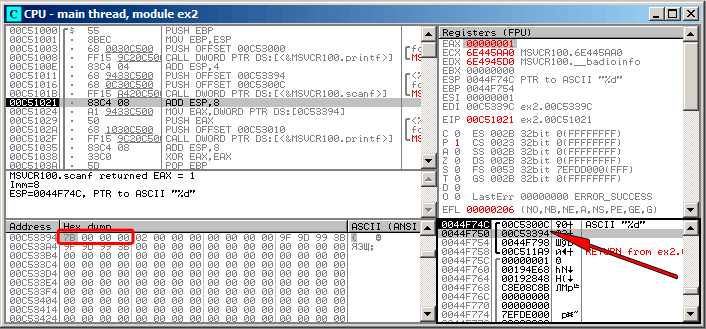
\includegraphics[scale=\FigScale]{patterns/04_scanf/2_global/ex2_olly_1.png}
\caption{\olly: after \scanf execution}
\label{fig:scanf_ex2_olly_1}
\end{figure}

The variable is located in the data segment.
After the \PUSH instruction (pushing the address of $x$) gets executed, 
the address appears in the stack window. Right-click on that row and select \q{Follow in dump}.
The variable will appear in the memory window on the left.
After we have entered 123 in the console, 
\TT{0x7B} appears in the memory window (see the highlighted screenshot regions).

But why is the first byte \TT{7B}?
Thinking logically, \TT{00 00 00 7B} should be
there.
The cause for this is referred as  \gls{endianness}, and x86 uses \IT{little-endian}.
This implies that the lowest byte is written first, and the highest written last.
Read more about it at: \myref{sec:endianness}.
Back to the example, the 32-bit value is loaded from this memory address into \EAX and passed to \printf.

The memory address of $x$ is \TT{0x00C53394}.

\clearpage
In \olly we can review the process memory map (Alt-M)
and we can see that this address is inside the \TT{.data} PE-segment of our program:

\begin{figure}[H]
\centering
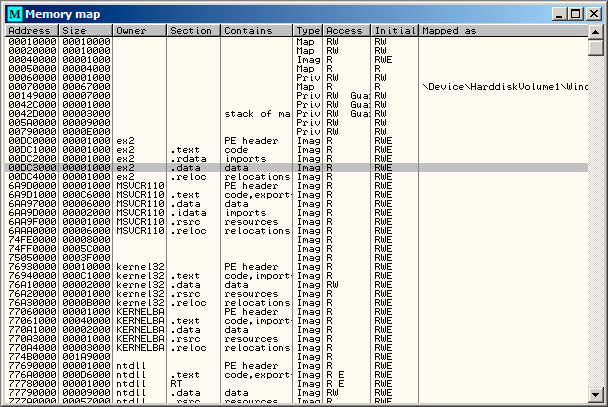
\includegraphics[scale=\FigScale]{patterns/04_scanf/2_global/ex2_olly_2.png}
\caption{\olly: process memory map}
\label{fig:scanf_ex2_olly_2}
\end{figure}

}
\RU{\clearpage
\subsectionold{MSVC: x86 + \olly}
\myindex{\olly}

Тут даже проще:

\begin{figure}[H]
\centering
\myincludegraphics{patterns/04_scanf/2_global/ex2_olly_1.png}
\caption{\olly: после исполнения \scanf}
\label{fig:scanf_ex2_olly_1}
\end{figure}

Переменная хранится в сегменте данных.
Кстати, после исполнения инструкции \PUSH (заталкивающей адрес $x$) адрес появится в стеке, 
и на этом элементе можно нажать правой кнопкой, выбрать \q{Follow in dump}.
И в окне памяти слева появится эта переменная.

После того как в консоли введем 123, здесь появится \TT{0x7B}.

Почему самый первый байт это \TT{7B}?
По логике вещей, здесь должно было бы быть \TT{00 00 00 7B}.
Это называется \gls{endianness}, и в x86 принят формат \IT{little-endian}.
Это означает, что в начале записывается самый младший байт, а заканчивается самым старшим байтом.
Больше об этом: \myref{sec:endianness}.

Позже из этого места в памяти 32-битное значение загружается в \EAX и передается в \printf.

Адрес переменной $x$ в памяти \TT{0x00C53394}.

\clearpage
В \olly{} мы можем посмотреть карту памяти процесса (Alt-M) и увидим, что этот адрес
внутри PE-сегмента \TT{.data} нашей программы:

\begin{figure}[H]
\centering
\myincludegraphics{patterns/04_scanf/2_global/ex2_olly_2.png}
\caption{\olly: карта памяти процесса}
\label{fig:scanf_ex2_olly_2}
\end{figure}
}
\ITA{\clearpage
\subsectionold{MSVC: x86 + \olly}
\myindex{\olly}

Il quadro qui è ancora più semplice:

\begin{figure}[H]
\centering
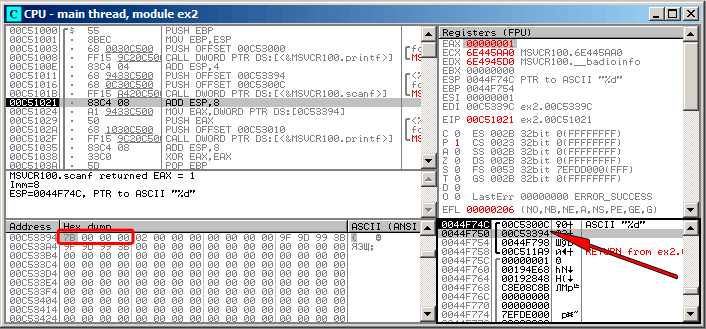
\includegraphics[scale=\FigScale]{patterns/04_scanf/2_global/ex2_olly_1.png}
\caption{\olly: after \scanf execution}
\label{fig:scanf_ex2_olly_1}
\end{figure}

La variabile è collocata nel data segment.
Dopo che l'istruzione \PUSH (che fa il push dell'indirizzo di $x$) viene eseguita, 
l'indirizzo appare nella finestra dello stack. Facciamo click destro su quella riga e selezioniamo \q{Follow in dump}.
La variabile apparirà nella finestra di memoria a sinistra.
Dopo aver inserito il valore 123 in console, 
\TT{0x7B} apparirà nella finestra della memoria (vedere regioni evidenziate nello screenshot).

Ma perchè il primo byte è \TT{7B}?
A rigor di logica, dovremmo trovare \TT{00 00 00 7B}.
La causa per cui troviamo invece \TT{7B} è detta \gls{endianness}, e x86 usa la convenzione \IT{little-endian}.
Ciò significa che il byte piu basso è scritto per primo, e quello più alto per ultimo.
Maggiori informazioni sono disponibili nella sezione: \myref{sec:endianness}.
Tornando all'esempio, il valore a 32-bit è caricato da questo indirizzo di memoria in \EAX e passato a \printf.

L'indirizzo in memoria di $x$ è \TT{0x00C53394}.

\clearpage
In \olly possiamo osservare la mappa di memoria di un processo  (process memory map, Alt-M)
e notare che questo indirizzo è dentro il segmento PE \TT{.data} del nostro programma:

\begin{figure}[H]
\centering
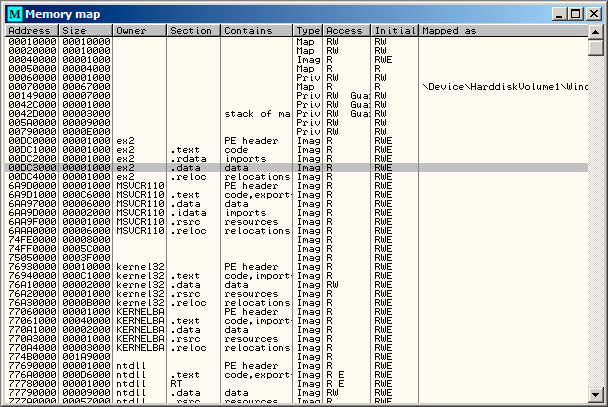
\includegraphics[scale=\FigScale]{patterns/04_scanf/2_global/ex2_olly_2.png}
\caption{\olly: process memory map}
\label{fig:scanf_ex2_olly_2}
\end{figure}

}


\subsectionold{GCC: x86}

\myindex{ELF}
The picture in Linux is near the same, with the difference that the uninitialized variables are located in the \TT{\_bss} segment. 
In \ac{ELF} file this segment has the following attributes:

\begin{lstlisting}
; Segment type: Uninitialized
; Segment permissions: Read/Write
\end{lstlisting}

If you, however, initialise the variable with some value e.g. 10, 
it is to be placed in the \TT{\_data} segment, which has the following attributes:

\begin{lstlisting}
; Segment type: Pure data
; Segment permissions: Read/Write
\end{lstlisting}

\subsectionold{MSVC: x64}

\lstinputlisting[caption=MSVC 2012 x64]{patterns/04_scanf/2_global/ex2_MSVC_x64_EN.asm}

The code is almost the same as in x86.
Please note that the address of the $x$ variable is passed to \TT{scanf()} using a \LEA instruction,
while the variable's value is passed to the second \printf using a \MOV instruction.
\TT{DWORD PTR}---is a part of the assembly language (no relation to the machine code),
indicating that the variable data size is 32-bit and the \MOV instruction has to be encoded accordingly.

}
\RU{\subsubsection{MSVC: x86}

\lstinputlisting{patterns/04_scanf/2_global/ex2_MSVC.asm}

В целом ничего особенного. Теперь \TT{x} объявлена в сегменте \TT{\_DATA}. 
Память для неё в стеке более не выделяется.
Все обращения к ней происходит не через стек, а уже напрямую. 
Неинициализированные глобальные переменные не занимают места в исполняемом файле
(и действительно, зачем в исполняемом файле
нужно выделять место под изначально нулевые переменные?), но тогда, когда к этому месту в памяти
кто-то обратится, \ac{OS} подставит туда блок, состоящий из нулей\footnote{Так работает \ac{VM}}.

Попробуем изменить объявление этой переменной:

\lstinputlisting{patterns/04_scanf/2_global/default_value_RU.c}

Выйдет в итоге:

\begin{lstlisting}
_DATA	SEGMENT
_x	DD	0aH

...
\end{lstlisting}

Здесь уже по месту этой переменной записано \TT{0xA} с типом DD (dword = 32 бита).

Если вы откроете скомпилированный .exe-файл в \IDA, то увидите, что \IT{x} 
находится в начале сегмента \TT{\_DATA}, после этой переменной будут текстовые строки.

А вот если вы откроете в \IDA .exe скомпилированный в прошлом примере, где значение \IT{x} не определено, то вы увидите:

\begin{lstlisting}
.data:0040FA80 _x              dd ?                    ; DATA XREF: _main+10
.data:0040FA80                                         ; _main+22
.data:0040FA84 dword_40FA84    dd ?                    ; DATA XREF: _memset+1E
.data:0040FA84                                         ; unknown_libname_1+28
.data:0040FA88 dword_40FA88    dd ?                    ; DATA XREF: ___sbh_find_block+5
.data:0040FA88                                         ; ___sbh_free_block+2BC
.data:0040FA8C ; LPVOID lpMem
.data:0040FA8C lpMem           dd ?                    ; DATA XREF: ___sbh_find_block+B
.data:0040FA8C                                         ; ___sbh_free_block+2CA
.data:0040FA90 dword_40FA90    dd ?                    ; DATA XREF: _V6_HeapAlloc+13
.data:0040FA90                                         ; __calloc_impl+72
.data:0040FA94 dword_40FA94    dd ?                    ; DATA XREF: ___sbh_free_block+2FE
\end{lstlisting}

\TT{\_x} обозначен как \TT{?}, наряду с другими переменными не требующими инициализации. 
Это означает, что при загрузке .exe в память, место под всё это выделено будет и будет заполнено
нулевыми байтами [\CNineNineStd 6.7.8p10]. 
Но в самом .exe ничего этого нет. Неинициализированные переменные не занимают места в исполняемых файлах. 
Это удобно для больших массивов, например.

\EN{\clearpage
\subsection{MSVC: x86 + \olly}
\myindex{\olly}

Things are even simpler here:

\begin{figure}[H]
\centering
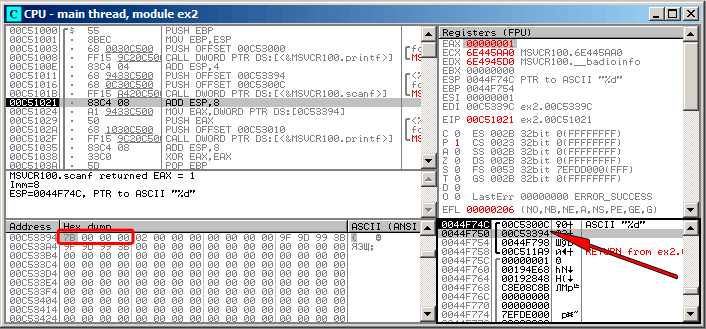
\includegraphics[scale=\FigScale]{patterns/04_scanf/2_global/ex2_olly_1.png}
\caption{\olly: after \scanf execution}
\label{fig:scanf_ex2_olly_1}
\end{figure}

The variable is located in the data segment.
After the \PUSH instruction (pushing the address of $x$) gets executed, 
the address appears in the stack window. Right-click on that row and select \q{Follow in dump}.
The variable will appear in the memory window on the left.
After we have entered 123 in the console, 
\TT{0x7B} appears in the memory window (see the highlighted screenshot regions).

But why is the first byte \TT{7B}?
Thinking logically, \TT{00 00 00 7B} should be
there.
The cause for this is referred as  \gls{endianness}, and x86 uses \IT{little-endian}.
This implies that the lowest byte is written first, and the highest written last.
Read more about it at: \myref{sec:endianness}.
Back to the example, the 32-bit value is loaded from this memory address into \EAX and passed to \printf.

The memory address of $x$ is \TT{0x00C53394}.

\clearpage
In \olly we can review the process memory map (Alt-M)
and we can see that this address is inside the \TT{.data} PE-segment of our program:

\begin{figure}[H]
\centering
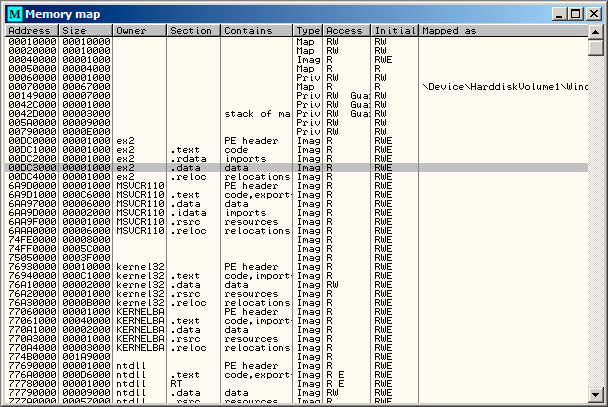
\includegraphics[scale=\FigScale]{patterns/04_scanf/2_global/ex2_olly_2.png}
\caption{\olly: process memory map}
\label{fig:scanf_ex2_olly_2}
\end{figure}

}
\RU{\clearpage
\subsectionold{MSVC: x86 + \olly}
\myindex{\olly}

Тут даже проще:

\begin{figure}[H]
\centering
\myincludegraphics{patterns/04_scanf/2_global/ex2_olly_1.png}
\caption{\olly: после исполнения \scanf}
\label{fig:scanf_ex2_olly_1}
\end{figure}

Переменная хранится в сегменте данных.
Кстати, после исполнения инструкции \PUSH (заталкивающей адрес $x$) адрес появится в стеке, 
и на этом элементе можно нажать правой кнопкой, выбрать \q{Follow in dump}.
И в окне памяти слева появится эта переменная.

После того как в консоли введем 123, здесь появится \TT{0x7B}.

Почему самый первый байт это \TT{7B}?
По логике вещей, здесь должно было бы быть \TT{00 00 00 7B}.
Это называется \gls{endianness}, и в x86 принят формат \IT{little-endian}.
Это означает, что в начале записывается самый младший байт, а заканчивается самым старшим байтом.
Больше об этом: \myref{sec:endianness}.

Позже из этого места в памяти 32-битное значение загружается в \EAX и передается в \printf.

Адрес переменной $x$ в памяти \TT{0x00C53394}.

\clearpage
В \olly{} мы можем посмотреть карту памяти процесса (Alt-M) и увидим, что этот адрес
внутри PE-сегмента \TT{.data} нашей программы:

\begin{figure}[H]
\centering
\myincludegraphics{patterns/04_scanf/2_global/ex2_olly_2.png}
\caption{\olly: карта памяти процесса}
\label{fig:scanf_ex2_olly_2}
\end{figure}
}
\ITA{\clearpage
\subsectionold{MSVC: x86 + \olly}
\myindex{\olly}

Il quadro qui è ancora più semplice:

\begin{figure}[H]
\centering
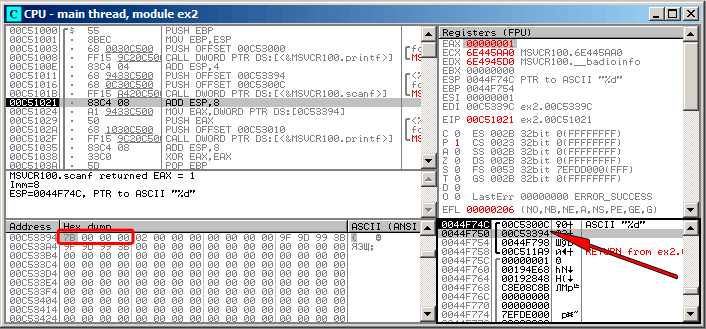
\includegraphics[scale=\FigScale]{patterns/04_scanf/2_global/ex2_olly_1.png}
\caption{\olly: after \scanf execution}
\label{fig:scanf_ex2_olly_1}
\end{figure}

La variabile è collocata nel data segment.
Dopo che l'istruzione \PUSH (che fa il push dell'indirizzo di $x$) viene eseguita, 
l'indirizzo appare nella finestra dello stack. Facciamo click destro su quella riga e selezioniamo \q{Follow in dump}.
La variabile apparirà nella finestra di memoria a sinistra.
Dopo aver inserito il valore 123 in console, 
\TT{0x7B} apparirà nella finestra della memoria (vedere regioni evidenziate nello screenshot).

Ma perchè il primo byte è \TT{7B}?
A rigor di logica, dovremmo trovare \TT{00 00 00 7B}.
La causa per cui troviamo invece \TT{7B} è detta \gls{endianness}, e x86 usa la convenzione \IT{little-endian}.
Ciò significa che il byte piu basso è scritto per primo, e quello più alto per ultimo.
Maggiori informazioni sono disponibili nella sezione: \myref{sec:endianness}.
Tornando all'esempio, il valore a 32-bit è caricato da questo indirizzo di memoria in \EAX e passato a \printf.

L'indirizzo in memoria di $x$ è \TT{0x00C53394}.

\clearpage
In \olly possiamo osservare la mappa di memoria di un processo  (process memory map, Alt-M)
e notare che questo indirizzo è dentro il segmento PE \TT{.data} del nostro programma:

\begin{figure}[H]
\centering
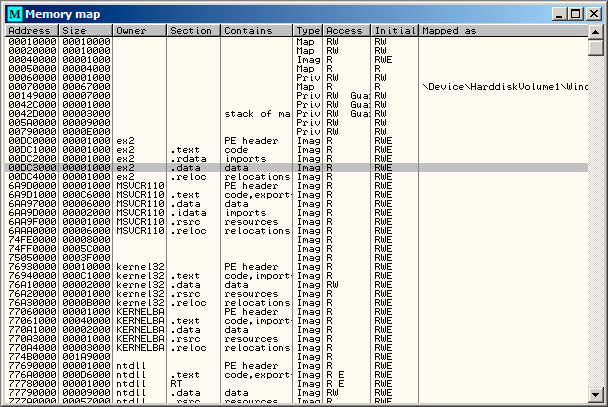
\includegraphics[scale=\FigScale]{patterns/04_scanf/2_global/ex2_olly_2.png}
\caption{\olly: process memory map}
\label{fig:scanf_ex2_olly_2}
\end{figure}

}


\subsubsection{GCC: x86}

\myindex{ELF}
В Linux всё почти также. За исключением того, что если значение \TT{x} не определено, 
то эта переменная будет находится в сегменте \TT{\_bss}.
В \ac{ELF} этот сегмент имеет такие атрибуты:

\begin{lstlisting}
; Segment type: Uninitialized
; Segment permissions: Read/Write
\end{lstlisting}

Ну а если сделать статическое присвоение этой переменной какого-либо
значения, например, 10, то она будет находится 
в сегменте \TT{\_data},
это сегмент с такими атрибутами:

\begin{lstlisting}
; Segment type: Pure data
; Segment permissions: Read/Write
\end{lstlisting}

\subsubsection{MSVC: x64}

\lstinputlisting[caption=MSVC 2012 x64]{patterns/04_scanf/2_global/ex2_MSVC_x64_RU.asm}

Почти такой же код как и в x86.
Обратите внимание что для \TT{scanf()} адрес переменной $x$ передается
при помощи инструкции \LEA, а во второй \printf передается само значение переменной при помощи \MOV.
\TT{DWORD PTR} --- это часть языка ассемблера (не имеющая отношения к машинным кодам) показывающая, что тип переменной в памяти именно 32-битный, 
и инструкция \MOV должна быть здесь закодирована соответственно.

}
\PTBR{\subsection{MSVC: x86}

\lstinputlisting{patterns/04_scanf/2_global/ex2_MSVC.asm}

Nesse caso, a variável \TT{x} é definida no segmento \TT{\_DATA} e nenhuma memória é alocada na pilha local.
Ela é acessada diretamente, não através da pilha.
Variáveis globais não inicialiadas não ocupam espaço no arquivo executável 
(realmente, ninguém precisa alocar espaço para uma variável inicialmente valendo zero), 
mas quando alguém acessa o endereço delas, o sistema operacional vai alocar um bloco contendo somente zeros nele.
\footnote{\ac{TBT}: That is how a \ac{VM} behaves}.

Agora vamos definir um valor para a variável:

% TODO translate
\lstinputlisting{patterns/04_scanf/2_global/default_value_EN.c}

Nós temos:

\begin{lstlisting}
_DATA	SEGMENT
_x	DD	0aH

...
\end{lstlisting}

Aqui nós vemos um valor \TT{0xA} do tipo DWORD (DD significa DWORD = 32 bits) para essa variável.

Se você abrir o .exe compilado no \IDA, você pode ver a variável \IT{x} colocada no começo do segmento \TT{\_DATA},
e depois disso você pode ver as strings.

Se você abrir o .exe compilado no exemplo anterior no \IDA, onde o valor de x não foi declarado, você poderá ver algo assim:

\begin{lstlisting}
.data:0040FA80 _x              dd ?                    ; DATA XREF: _main+10
.data:0040FA80                                         ; _main+22
.data:0040FA84 dword_40FA84    dd ?                    ; DATA XREF: _memset+1E
.data:0040FA84                                         ; unknown_libname_1+28
.data:0040FA88 dword_40FA88    dd ?                    ; DATA XREF: ___sbh_find_block+5
.data:0040FA88                                         ; ___sbh_free_block+2BC
.data:0040FA8C ; LPVOID lpMem
.data:0040FA8C lpMem           dd ?                    ; DATA XREF: ___sbh_find_block+B
.data:0040FA8C                                         ; ___sbh_free_block+2CA
.data:0040FA90 dword_40FA90    dd ?                    ; DATA XREF: _V6_HeapAlloc+13
.data:0040FA90                                         ; __calloc_impl+72
.data:0040FA94 dword_40FA94    dd ?                    ; DATA XREF: ___sbh_free_block+2FE
\end{lstlisting}

\TT{\_x} está marcada com \TT{?} juntamente com o resto das variáveis que não precisam ser inicializadas.
Isso implica que após carregar o .exe para a memória, um espaço para todas essas variáveis será alocado e preenchido com zeros [\CNineNineStd 6.7.8p10].
Mas no arquivo .exe essas variáveis não inicializadas não ocupam nenhum espaço.
Isso é conveniente para arrays grandes, por exemplo.

\EN{\clearpage
\subsection{MSVC: x86 + \olly}
\myindex{\olly}

Things are even simpler here:

\begin{figure}[H]
\centering
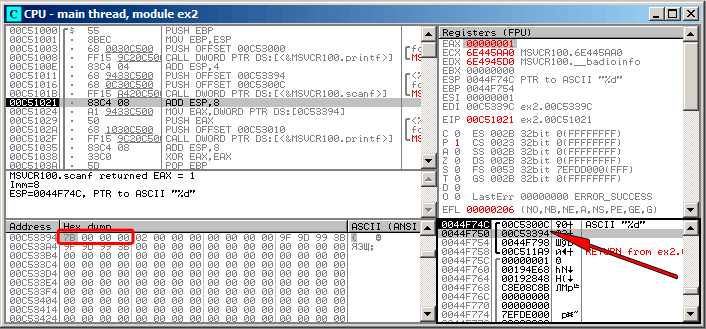
\includegraphics[scale=\FigScale]{patterns/04_scanf/2_global/ex2_olly_1.png}
\caption{\olly: after \scanf execution}
\label{fig:scanf_ex2_olly_1}
\end{figure}

The variable is located in the data segment.
After the \PUSH instruction (pushing the address of $x$) gets executed, 
the address appears in the stack window. Right-click on that row and select \q{Follow in dump}.
The variable will appear in the memory window on the left.
After we have entered 123 in the console, 
\TT{0x7B} appears in the memory window (see the highlighted screenshot regions).

But why is the first byte \TT{7B}?
Thinking logically, \TT{00 00 00 7B} should be
there.
The cause for this is referred as  \gls{endianness}, and x86 uses \IT{little-endian}.
This implies that the lowest byte is written first, and the highest written last.
Read more about it at: \myref{sec:endianness}.
Back to the example, the 32-bit value is loaded from this memory address into \EAX and passed to \printf.

The memory address of $x$ is \TT{0x00C53394}.

\clearpage
In \olly we can review the process memory map (Alt-M)
and we can see that this address is inside the \TT{.data} PE-segment of our program:

\begin{figure}[H]
\centering
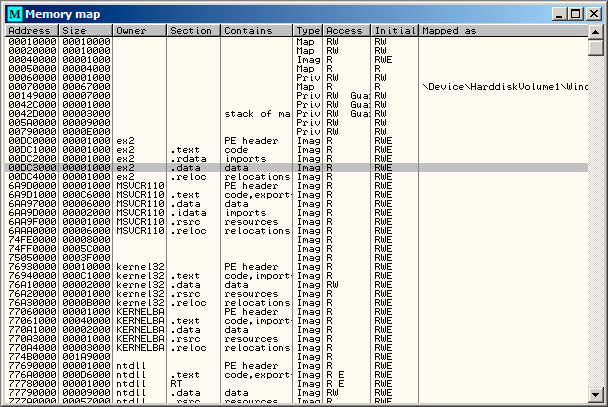
\includegraphics[scale=\FigScale]{patterns/04_scanf/2_global/ex2_olly_2.png}
\caption{\olly: process memory map}
\label{fig:scanf_ex2_olly_2}
\end{figure}

}
\RU{\clearpage
\subsectionold{MSVC: x86 + \olly}
\myindex{\olly}

Тут даже проще:

\begin{figure}[H]
\centering
\myincludegraphics{patterns/04_scanf/2_global/ex2_olly_1.png}
\caption{\olly: после исполнения \scanf}
\label{fig:scanf_ex2_olly_1}
\end{figure}

Переменная хранится в сегменте данных.
Кстати, после исполнения инструкции \PUSH (заталкивающей адрес $x$) адрес появится в стеке, 
и на этом элементе можно нажать правой кнопкой, выбрать \q{Follow in dump}.
И в окне памяти слева появится эта переменная.

После того как в консоли введем 123, здесь появится \TT{0x7B}.

Почему самый первый байт это \TT{7B}?
По логике вещей, здесь должно было бы быть \TT{00 00 00 7B}.
Это называется \gls{endianness}, и в x86 принят формат \IT{little-endian}.
Это означает, что в начале записывается самый младший байт, а заканчивается самым старшим байтом.
Больше об этом: \myref{sec:endianness}.

Позже из этого места в памяти 32-битное значение загружается в \EAX и передается в \printf.

Адрес переменной $x$ в памяти \TT{0x00C53394}.

\clearpage
В \olly{} мы можем посмотреть карту памяти процесса (Alt-M) и увидим, что этот адрес
внутри PE-сегмента \TT{.data} нашей программы:

\begin{figure}[H]
\centering
\myincludegraphics{patterns/04_scanf/2_global/ex2_olly_2.png}
\caption{\olly: карта памяти процесса}
\label{fig:scanf_ex2_olly_2}
\end{figure}
}
\ITA{\clearpage
\subsectionold{MSVC: x86 + \olly}
\myindex{\olly}

Il quadro qui è ancora più semplice:

\begin{figure}[H]
\centering
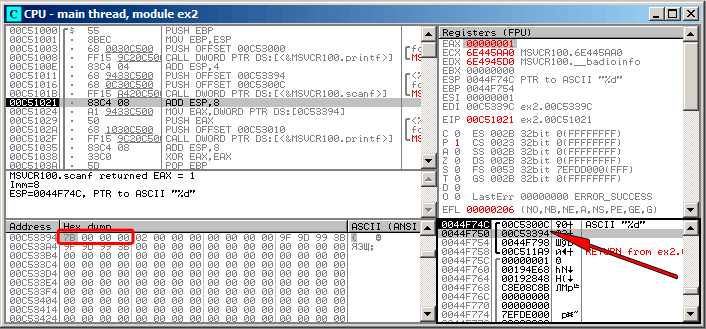
\includegraphics[scale=\FigScale]{patterns/04_scanf/2_global/ex2_olly_1.png}
\caption{\olly: after \scanf execution}
\label{fig:scanf_ex2_olly_1}
\end{figure}

La variabile è collocata nel data segment.
Dopo che l'istruzione \PUSH (che fa il push dell'indirizzo di $x$) viene eseguita, 
l'indirizzo appare nella finestra dello stack. Facciamo click destro su quella riga e selezioniamo \q{Follow in dump}.
La variabile apparirà nella finestra di memoria a sinistra.
Dopo aver inserito il valore 123 in console, 
\TT{0x7B} apparirà nella finestra della memoria (vedere regioni evidenziate nello screenshot).

Ma perchè il primo byte è \TT{7B}?
A rigor di logica, dovremmo trovare \TT{00 00 00 7B}.
La causa per cui troviamo invece \TT{7B} è detta \gls{endianness}, e x86 usa la convenzione \IT{little-endian}.
Ciò significa che il byte piu basso è scritto per primo, e quello più alto per ultimo.
Maggiori informazioni sono disponibili nella sezione: \myref{sec:endianness}.
Tornando all'esempio, il valore a 32-bit è caricato da questo indirizzo di memoria in \EAX e passato a \printf.

L'indirizzo in memoria di $x$ è \TT{0x00C53394}.

\clearpage
In \olly possiamo osservare la mappa di memoria di un processo  (process memory map, Alt-M)
e notare che questo indirizzo è dentro il segmento PE \TT{.data} del nostro programma:

\begin{figure}[H]
\centering
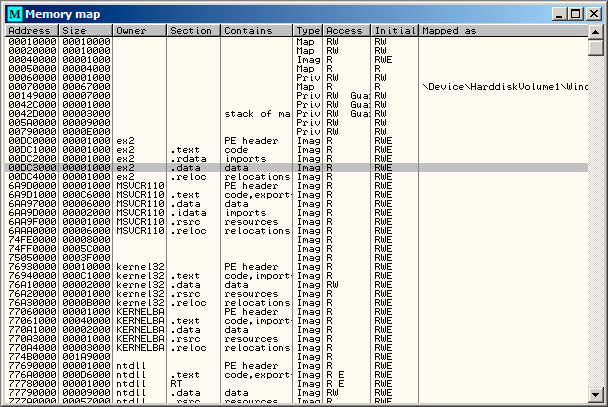
\includegraphics[scale=\FigScale]{patterns/04_scanf/2_global/ex2_olly_2.png}
\caption{\olly: process memory map}
\label{fig:scanf_ex2_olly_2}
\end{figure}

}


\subsection{GCC: x86}

\PTBRph{}

\subsection{MSVC: x64}

% TODO translate
\lstinputlisting[caption=MSVC 2012 x64]{patterns/04_scanf/2_global/ex2_MSVC_x64_EN.asm}

O código é quase o mesmo que no x86.
Por favor, perceba que o endereço da variável x é passado para \TT{scanf()} usando uma instrução \LEA,
enquanto os valores das variáveis são passadas para o segundo \printf usando uma instrução \MOV.
\TT{DWORD PTR} é uma parte da linguagem assembly (sem relação com o código de máquina),
indicando que o tamanho da informação da variável é de 32-bits e que a instrução \MOV tem de ser codificada de acordo.

}
\ifdefined\IncludeARM
\EN{\subsection{ARM: \OptimizingKeilVI (\ThumbMode)}

\begin{lstlisting}
.text:00000000 ; Segment type: Pure code
.text:00000000                 AREA .text, CODE
...
.text:00000000 main
.text:00000000                 PUSH    {R4,LR}
.text:00000002                 ADR     R0, aEnterX     ; "Enter X:\n"
.text:00000004                 BL      __2printf
.text:00000008                 LDR     R1, =x
.text:0000000A                 ADR     R0, aD          ; "%d"
.text:0000000C                 BL      __0scanf
.text:00000010                 LDR     R0, =x
.text:00000012                 LDR     R1, [R0]
.text:00000014                 ADR     R0, aYouEnteredD___ ; "You entered %d...\n"
.text:00000016                 BL      __2printf
.text:0000001A                 MOVS    R0, #0
.text:0000001C                 POP     {R4,PC}
...
.text:00000020 aEnterX         DCB "Enter X:",0xA,0    ; DATA XREF: main+2
.text:0000002A                 DCB    0
.text:0000002B                 DCB    0
.text:0000002C off_2C          DCD x                   ; DATA XREF: main+8
.text:0000002C                                         ; main+10
.text:00000030 aD              DCB "%d",0              ; DATA XREF: main+A
.text:00000033                 DCB    0
.text:00000034 aYouEnteredD___ DCB "You entered %d...",0xA,0 ; DATA XREF: main+14
.text:00000047                 DCB 0
.text:00000047 ; .text         ends
.text:00000047
...
.data:00000048 ; Segment type: Pure data
.data:00000048                 AREA .data, DATA
.data:00000048                 ; ORG 0x48
.data:00000048                 EXPORT x
.data:00000048 x               DCD 0xA                 ; DATA XREF: main+8
.data:00000048                                         ; main+10
.data:00000048 ; .data         ends
\end{lstlisting}

So, the \TT{x} variable is now global and for this reason located in another segment, namely the data segment (\IT{.data}).
One could ask, why are the text strings located in the code segment (\IT{.text}) and \TT{x} is located right here?
Because it is a variable and by definition its value could change. Moreover it could possibly change often.
While text strings has constant type, they will not be changed, so they are located in the \IT{.text} segment.
\myindex{\RAM}
\myindex{\ROM}

The code segment might sometimes be located in a \ac{ROM} chip (remember, we now deal
with embedded microelectronics, and memory scarcity is common here), and changeable 
variables~---in \ac{RAM}.

It is not very economical to store constant variables in RAM when you have ROM.

Furthermore, constant variables in RAM must be initialized, because after powering on, the RAM, obviously, contains random information.

\myindex{Linker}

Moving forward, we see a pointer to the \TT{x} (\TT{off\_2C}) variable in the code segment, and that all
operations with the variable occur via this pointer.

That is because the \TT{x} variable could be located somewhere far from this particular code fragment, so its address
must be saved somewhere in close proximity to the code.
\myindex{ARM!\Instructions!LDR}

The \INS{LDR} instruction in Thumb mode can only address variables in a range of 1020 bytes from its location, 

and in in ARM-mode~---variables in range of $\pm{}4095$ bytes.

And so the address of the \TT{x} variable
must be located somewhere in close proximity, because there is no guarantee that the linker would be able to accommodate the variable somewhere nearby the code, it may well be even in an external memory chip!

\myindex{\CLanguageElements!const}
\myindex{\ROM}

One more thing: if a variable is declared as \IT{const}, the Keil compiler allocates it in 
the \TT{.constdata} segment.

Perhaps thereafter, the linker could place this segment in ROM too, along with the code segment.

\subsection{ARM64}

\lstinputlisting[caption=\NonOptimizing GCC 4.9.1 ARM64,numbers=left]{patterns/04_scanf/2_global/ARM64_GCC491_O0.s.\LANG}

\myindex{ARM!\Instructions!ADRP/ADD pair}

In this case the $x$ variable is declared as global and its address is calculated using 
the \INS{ADRP}/\INS{ADD} instruction pair (lines 21 and 25).

}
\RU{\subsection{ARM: \OptimizingKeilVI (\ThumbMode)}

\begin{lstlisting}
.text:00000000 ; Segment type: Pure code
.text:00000000                 AREA .text, CODE
...
.text:00000000 main
.text:00000000                 PUSH    {R4,LR}
.text:00000002                 ADR     R0, aEnterX     ; "Enter X:\n"
.text:00000004                 BL      __2printf
.text:00000008                 LDR     R1, =x
.text:0000000A                 ADR     R0, aD          ; "%d"
.text:0000000C                 BL      __0scanf
.text:00000010                 LDR     R0, =x
.text:00000012                 LDR     R1, [R0]
.text:00000014                 ADR     R0, aYouEnteredD___ ; "You entered %d...\n"
.text:00000016                 BL      __2printf
.text:0000001A                 MOVS    R0, #0
.text:0000001C                 POP     {R4,PC}
...
.text:00000020 aEnterX         DCB "Enter X:",0xA,0    ; DATA XREF: main+2
.text:0000002A                 DCB    0
.text:0000002B                 DCB    0
.text:0000002C off_2C          DCD x                   ; DATA XREF: main+8
.text:0000002C                                         ; main+10
.text:00000030 aD              DCB "%d",0              ; DATA XREF: main+A
.text:00000033                 DCB    0
.text:00000034 aYouEnteredD___ DCB "You entered %d...",0xA,0 ; DATA XREF: main+14
.text:00000047                 DCB 0
.text:00000047 ; .text         ends
.text:00000047
...
.data:00000048 ; Segment type: Pure data
.data:00000048                 AREA .data, DATA
.data:00000048                 ; ORG 0x48
.data:00000048                 EXPORT x
.data:00000048 x               DCD 0xA                 ; DATA XREF: main+8
.data:00000048                                         ; main+10
.data:00000048 ; .data         ends
\end{lstlisting}

Итак, переменная \TT{x} теперь глобальная, и она расположена, почему-то, в другом сегменте, а именно сегменте данных (\IT{.data}).
Можно спросить, почему текстовые строки расположены в сегменте кода (\IT{.text}), а \TT{x} нельзя было разместить тут же?

Потому что эта переменная, и как следует из определения, она может меняться. И может быть, меняться часто.

Ну а текстовые строки имеют тип констант, они не будут меняться, поэтому они располагаются в сегменте \IT{.text}.

\myindex{\RAM}
\myindex{\ROM}
Сегмент кода иногда может быть расположен в ПЗУ микроконтроллера (не забывайте, 
мы сейчас имеем дело с embedded-микроэлектроникой, где дефицит памяти~--- обычное дело),
а изменяемые переменные~--- в ОЗУ.

Хранить в ОЗУ неизменяемые данные, когда в наличии есть ПЗУ, не экономно.

К тому же, сегмент данных в ОЗУ с константами нужно инициализировать перед работой,
ведь, после включения ОЗУ, очевидно, она содержит в себе случайную информацию.

\myindex{Компоновщик}
Далее мы видим в сегменте кода хранится указатель на переменную \TT{x} (\TT{off\_2C}) и 
все операции с переменной происходят через этот указатель.

Это связано с тем, что переменная \TT{x} может быть расположена где-то довольно далеко от 
данного участка кода, так что её адрес нужно сохранить в непосредственной близости к этому коду.

\myindex{ARM!\Instructions!LDR}
Инструкция \INS{LDR} в Thumb-режиме может адресовать только переменные в пределах вплоть до 1020 байт от своего местоположения.

Эта же инструкция в ARM-режиме~--- переменные в пределах $\pm{}4095$ байт.

Таким образом,
адрес глобальной переменной \TT{x} нужно расположить в непосредственной близости, ведь нет никакой гарантии, 
что компоновщик\footnote{linker в англоязычной литературе} сможет разместить саму переменную где-то рядом, 
она может быть даже в другом чипе памяти!

\myindex{\CLanguageElements!const}
\myindex{\ROM}
Ещё одна вещь: если переменную объявить как \IT{const}, то компилятор Keil разместит её в сегменте \TT{.constdata}.

Должно быть, впоследствии компоновщик и этот сегмент сможет разместить в ПЗУ вместе с сегментом кода.

\subsection{ARM64}

\lstinputlisting[caption=\NonOptimizing GCC 4.9.1 ARM64,numbers=left]{patterns/04_scanf/2_global/ARM64_GCC491_O0.s.\LANG}

\myindex{ARM!\Instructions!ADRP/ADD pair}
Теперь $x$ это глобальная переменная, и её адрес вычисляется при помощи пары инструкций \INS{ADRP}/\INS{ADD} (строки 21 и 25).

}
\fi
\ifdefined\IncludeMIPS
\EN{\subsection{MIPS}

\subsubsection{Uninitialized global variable}

So now the $x$ variable is global.
Let's compile to executable file rather than object file and load it into \IDA.
IDA displays the $x$ variable in the .sbss ELF section (remember the \q{Global Pointer}? \myref{MIPS_GP}),
since the variable is not initialized at the start.

\lstinputlisting[caption=\Optimizing GCC 4.4.5 (IDA)]{patterns/04_scanf/2_global/MIPS/O3_IDA.lst.\LANG}

IDA reduces the amount of information, so we'll also do a listing using objdump and comment it:

\lstinputlisting[caption=\Optimizing GCC 4.4.5 (objdump),numbers=left]{patterns/04_scanf/2_global/MIPS/O3_objdump.txt.\LANG}

Now we see the $x$ variable address is read from a 64KiB data buffer using GP and adding negative offset to it (line 18).
More than that, the addresses of the three external functions  which are used in our example (\puts, \scanf, \printf), are also read from the 64KiB global data buffer using GP (lines 9, 16 and 26).
GP points to the middle of the buffer, and such offset suggests that all three function's addresses,
and also the address of the $x$ variable, are all stored somewhere at the beginning of that buffer.
That make sense, because our example is tiny.

\myindex{MIPS!\Pseudoinstructions!MOVE}
\myindex{MIPS!\Pseudoinstructions!NOP}

Another thing worth mentioning is that the function ends with two \ac{NOP}s (\TT{MOVE \$AT,\$AT} --- an idle instruction), in order to align next function's start on 16-byte boundary.

\subsubsection{Initialized global variable}

Let's alter our example by giving the $x$ variable a default value:

\lstinputlisting{patterns/04_scanf/2_global/default_value.c.\LANG}

Now IDA shows that the $x$ variable is residing in the .data section:

\lstinputlisting[caption=\Optimizing GCC 4.4.5 (IDA)]{patterns/04_scanf/2_global/MIPS/O3_IDA_init.lst.\LANG}

Why not .sdata? Perhaps that this depends on some GCC option?

Nevertheless, now $x$ is in .data, which is a general memory area, and we can take a look
how to work with variables there.

\myindex{MIPS!\Instructions!LUI}
\myindex{MIPS!\Instructions!ADDIU}

The variable's address must be formed using a pair of instructions.

In our case those are \INS{LUI} (\q{Load Upper Immediate}) and \INS{ADDIU} (\q{Add Immediate Unsigned Word}).

Here is also the objdump listing for close inspection:

\lstinputlisting[caption=\Optimizing GCC 4.4.5 (objdump)]{patterns/04_scanf/2_global/MIPS/O3_objdump_init.txt.\LANG}

\myindex{MIPS!\Instructions!LUI}
\myindex{MIPS!\Instructions!ADDIU}
\myindex{MIPS!\Instructions!LW}

We see that the address is formed using \INS{LUI} and \INS{ADDIU}, but the high part of address is still in
the \$S0 register, and it is possible to encode the offset in a \INS{LW} (\q{Load Word}) instruction, so one single \INS{LW} is enough 
to load a value from the variable and pass it to \printf.

Registers holding temporary data are prefixed with T-, but here we also see some prefixed with S-, 
the contents of which is need to be preserved before use in other functions (i.e., \q{saved}).
% FIXME:
% This needs to be clarified a bit, e.g. "the registers need to be preserved if a function is called and it wants to use them

That is why the value of \$S0 was set at address 0x4006cc and was used again
at address 0x4006e8, after the \scanf call. 
The \scanf function does not change its value.

% TODO non-optimized example?
}
\RU{\subsubsection{MIPS}

\myparagraph{Неинициализированная глобальная переменная}

Так что теперь переменная $x$ глобальная.
Сделаем исполняемый файл вместо объектного и загрузим его в \IDA.
IDA показывает присутствие переменной $x$ в ELF-секции .sbss (помните о \q{Global Pointer}? \myref{MIPS_GP}),
так как переменная не инициализируется в самом начале.

\lstinputlisting[caption=\Optimizing GCC 4.4.5 (IDA)]{patterns/04_scanf/2_global/MIPS/O3_IDA_RU.lst}

IDA уменьшает количество информации, так что сделаем также листинг используя objdump и добавим туда свои комментарии:

\lstinputlisting[caption=\Optimizing GCC 4.4.5 (objdump),numbers=left]{patterns/04_scanf/2_global/MIPS/O3_objdump_RU.txt}

Теперь мы видим, как адрес переменной $x$ берется из буфера 64KiB, используя GP и прибавление к нему отрицательного смещения (строка 18).

И даже более того: адреса трех внешних функций, используемых в нашем примере (\puts, \scanf, \printf)
также берутся из буфера 64KiB используя GP (строки 9, 16 и 26).

GP указывает на середину буфера, так что такие смещения могут нам подсказать, что адреса всех трех функций,
а также адрес переменной $x$ расположены где-то в самом начале буфера.
Действительно, ведь наш пример крохотный.

\myindex{MIPS!\Pseudoinstructions!MOVE}
\myindex{MIPS!\Pseudoinstructions!NOP}
Ещё нужно отметить что функция заканчивается двумя \ac{NOP}-ами (\TT{MOVE \$AT,\$AT}~--- 
это холостая инструкция), чтобы выровнять начало следующей функции по 16-байтной границе.

\myparagraph{Инициализированная глобальная переменная}

Немного изменим наш пример и сделаем, чтобы у $x$ было значение по умолчанию:

\lstinputlisting{patterns/04_scanf/2_global/default_value_RU.c}

Теперь IDA показывает что переменная $x$ располагается в секции .data:

\lstinputlisting[caption=\Optimizing GCC 4.4.5 (IDA)]{patterns/04_scanf/2_global/MIPS/O3_IDA_init_RU.lst}

Почему не .sdata? Может быть, нужно было указать какую-то опцию в GCC?
Тем не менее, $x$ теперь в .data, а это уже общая память и мы можем посмотреть как происходит
работа с переменными там.

\myindex{MIPS!\Instructions!LUI}
\myindex{MIPS!\Instructions!ADDIU}
Адрес переменной должен быть сформирован парой инструкций.
В нашем случае это \INS{LUI} (\q{Load Upper Immediate}~--- загрузить старшие 16 бит) и 
\INS{ADDIU} (\q{Add Immediate Unsigned Word}~--- прибавить значение).
Вот так же листинг сгенерированный objdump-ом для лучшего рассмотрения:

\lstinputlisting[caption=\Optimizing GCC 4.4.5 (objdump)]{patterns/04_scanf/2_global/MIPS/O3_objdump_init_RU.txt}

\myindex{MIPS!\Instructions!LUI}
\myindex{MIPS!\Instructions!ADDIU}
\myindex{MIPS!\Instructions!LW}
Адрес формируется используя \INS{LUI} и \INS{ADDIU}, но старшая часть адреса
всё ещё в регистре \$S0, и можно закодировать смещение в инструкции \INS{LW} (\q{Load Word}), так что одной
\INS{LW} достаточно для загрузки значения из переменной и передачи его в \printf.
Регистры хранящие временные данные имеют префикс T-, но здесь есть также регистры с префиксом S-,
содержимое которых должно быть сохранено в других функциях (т.е. \q{saved}).

% FIXME:
% This needs to be clarified a bit, e.g. "the registers need to be preserved if a function is called and it wants to use them
Вот почему \$S0 был установлен по адресу 0x4006cc и затем был использован по адресу 0x4006e8
после вызова \scanf.

Функция \scanf не изменяет это значение.

% TODO non-optimized example?
}


\fi
